\chapter{随机向量及常见分布}
\begin{introduction}
  \item Intro to Prob\quad2.5 \quad 3.4 
  \item Prob $\&$ Stat\quad3.1\quad3.2
\end{introduction}

\section{引导问题:一维 vs 多维}

当我们想要研究本学期某一个学生的概率论与数理统计的期末成绩,记其为$X_1$。显然,$X_1$是一个随机变量,其取值应该是从0至100之间的自然数。此时,我们并不知道期末考试成绩的分布,所以,我们也无法预测某一位同学的期末成绩。

值得注意的是,在课程大纲中,高等数学和线性代数列为概率论与数理统计的先修课程。记其高等数学的期末成绩为$X_2$,而线性代数的期末成绩为$X_3$。图\ref{fig:chap08_score_in_Probability_Statistics}是高等数学、线性代数分别与概率论与数理统计期末考试的散点图。

\begin{figure}[ht]
    \centering
    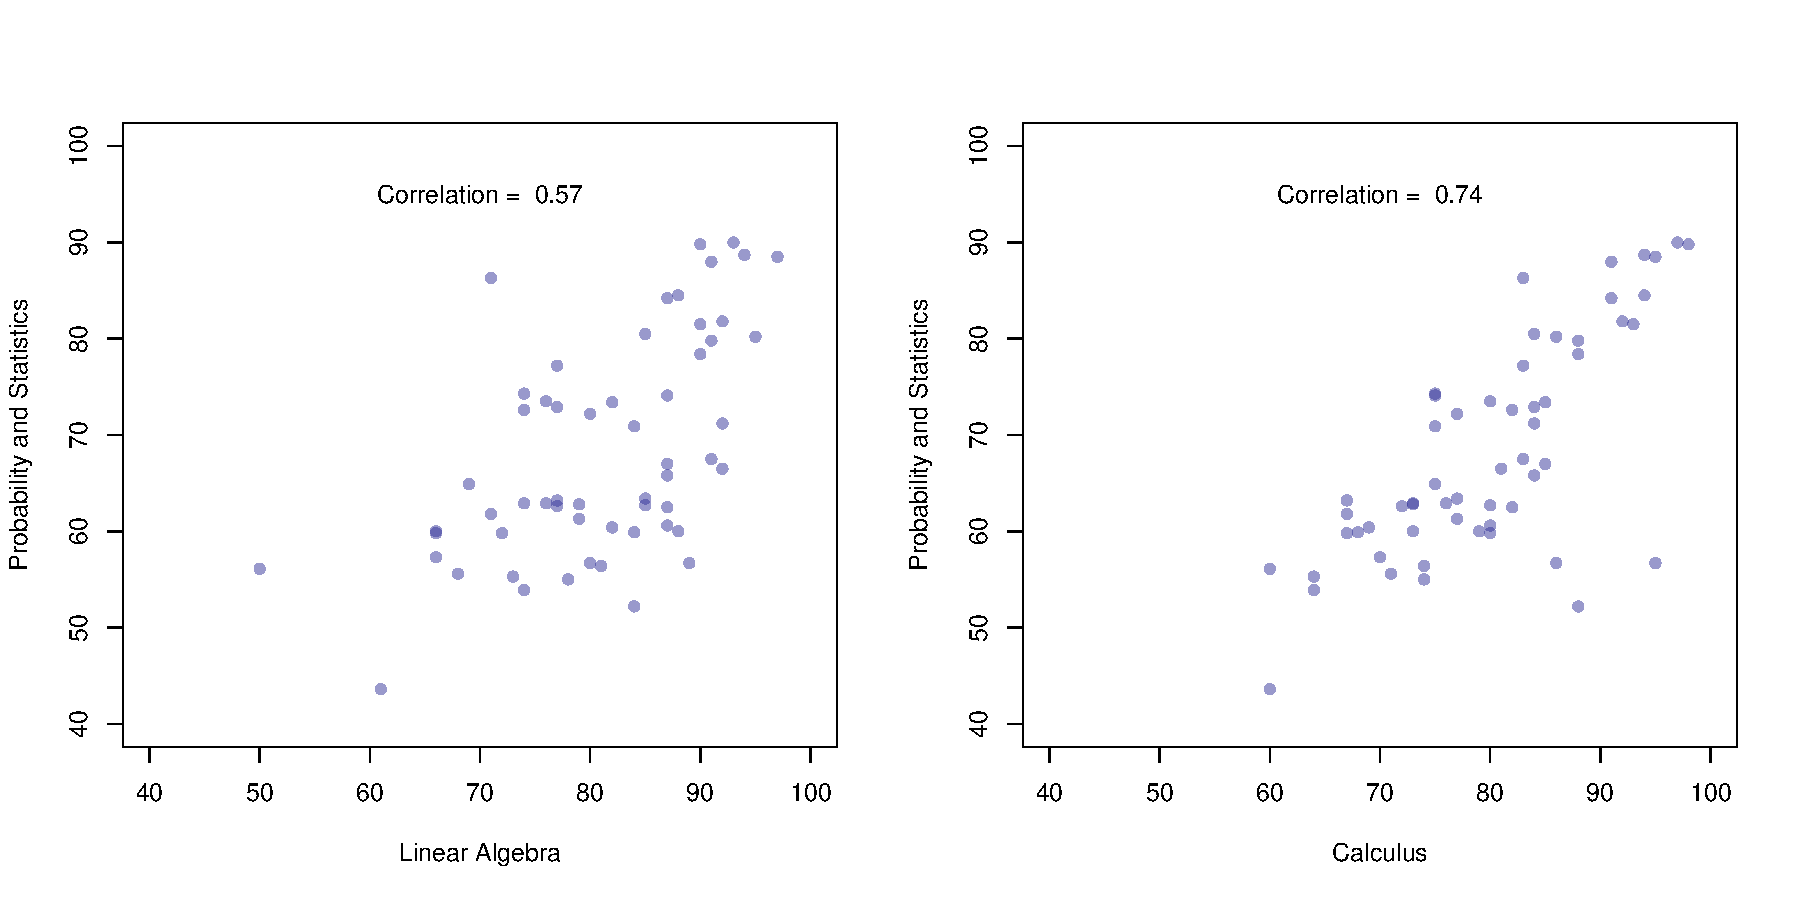
\includegraphics[width=0.75\linewidth]{image/Chap8_score_in_Probability_Statistics.pdf}
    \caption{两门先修课程与《概率论与数理统计》课程期末成绩的关系}
    \label{fig:chap08_score_in_Probability_Statistics}
\end{figure}

如果我们研究清楚$X_1,X_2,X_3$之间的关系,那么我们可以通过已知的$X_2$和$X_3$来预测未知的$X_1$。这就是一般建模的逻辑。因此,如何同时研究多个随机变量是必要的。


\section{随机向量的定义}
\begin{example}
\begin{enumerate}
    \item 大学生的身高$X_{1}(\omega)$和体重$X_{2}(\omega)$构成一个二维随机变量。
    \item 考虑大学生的一个月生活费,按衣、食、行及其他的支出,记为$X_{1}(\omega),X_{2}(\omega),X_{3}(\omega),X_{4}(\omega)$,其中,$\left(X_{1}, X_{2}, X_{3}, X_{4}\right)$ 就是一个四维随机变量。
\end{enumerate}
\end{example}

\begin{definition}{随机向量}
如果$X_{1}(\omega),X_{2}(\omega),...,X_{n}(\omega)$是定义在同一个样本空间$\Omega=\{\omega\}$上的$n$个随机变量,则称
$$\bm{X}(\omega)=\left(X_{1}(\omega), X_{2}(\omega), \ldots, X_{n}(\omega)\right)'$$
为$n$维(或$n$元)随机变量或随机向量。
\end{definition}

\begin{remark}
    所有定义的随机向量都是\textbf{列向量}。一维随机向量就是随机变量。
\end{remark}



\section{随机向量的联合分布函数}
\begin{definition}
对任意$n$个实数$x_{1}, x_{2}, \cdots, x_{n}$,$n$个事件$\left\{X_{1} \leqslant x_{1}\right\},\left\{X_{2} \leqslant x_{2}\right\},...,\left\{X_{n} \leqslant x_{n}\right\}$同时发生的概率
\begin{eqnarray*}
F\left(x_{1}, x_{2}, \cdots, x_{n}\right)&=&P\left( \{X_{1} \leqslant x_{1}\} \cap \{X_{2} \leqslant x_{2}\}\cap \cdots\cap \{X_{n} \leqslant x_{n}\}\right)\\
&=& P\left(X_{1} \leq x_1, X_2 \leq x_2,\cdots,X_n \leq x_{n}\right)
\end{eqnarray*}
称为$n$维随机向量$\bm{X}$的联合分布函数。
\end{definition}
\begin{remark}
    对于二维随机向量$(X,Y)'$,其联合分布函数为
    $$
    F(x,y) = P(X\leq x, Y\leq y)
    $$
\end{remark}

\begin{theorem}{二维随机变量联合分布函数的性质}\label{thm: property_of_two_dim_rv}
任一二维联合分布函数$F(x,y)$必具有如下性质:
\begin{enumerate}
    \item \textbf{单调性}:$F(x,y)$分别对$x$或$y$是单调非减的,即
    
    当$x_{1}<x_{2}$时,有$$F\left(x_{1}, y\right) \leq F\left(x_{2}, y\right);$$
    当$y_{1}<y_{2}$时,有
    $$F\left(x, y_{1}\right) \leq F\left(x, y_{2}\right).$$
    \item \textbf{有界性}:对任意的$x$和y,有$0 \leqslant F(x, y) \leqslant 1$且
    \begin{eqnarray*}
        F(-\infty, y)&=&\lim _{x \rightarrow-\infty} F(x, y)=0, \\
F(x,-\infty)&=&\lim _{y \rightarrow-\infty} F(x, y)=0, \\
F(\infty, \infty)&=&\lim _{x, y \rightarrow \infty} F(x, y)=1.
    \end{eqnarray*}
    \item \textbf{右连续性}:对每个变量都是右连续的,即
    \begin{eqnarray*}
        F(x+0, y)&=&F(x, y) \\
F(x, y+0)&=&F(x, y)
    \end{eqnarray*}
    \item \textbf{非负性}:对任意的$a<b,c<d$有
    \begin{eqnarray*}
        P(a<X \leq b, c<Y \leqslant d) &=&F(b, d)-F(a, d)-F(b, c)+F(a, c)  \geqslant 0
    \end{eqnarray*}
\end{enumerate}
\end{theorem}

\begin{remark}
\begin{enumerate}
    \item 具有以上四条性质的二元函数$F(x,y)$一定是某个二维随机变量的分布函数。
    \item 性质(4)是二维随机向量所特有的,也是合理的,但性质(4)不能由前三条性质推出,因此需要单独列出。
\end{enumerate}
\end{remark}
\begin{example}
    设二元函数为
    $$G(x, y)=\left\{\begin{array}{ll}
0 & x+y<0 \\
1 & x+y \geqslant 0
\end{array}\right. $$
可以证明其满足前三个性质(这里留给学生课后完成),但该函数不满足性质4。考虑在$(-1,-1),(1,-1),(-1,1),(1,1)$所围成的正方形上的面积。
\end{example}
\begin{note}
   \vspace{5cm} 
\end{note}

\section{边际分布函数}
\begin{definition}{边际分布函数}\label{def:m.c.d.f}
    如果二维随机变量$(X,Y)$的联合分布函数为$F(x,y)$,那么,称
    $$F_X(x) = P(X\leq x) = P(X\leq x, Y< \infty) = \lim_{y\rightarrow \infty} F(x,y)$$
    为$X$的边际分布。
    类似地,称
    $$
    F_Y(y) = F(\infty,y)
    $$
    为$Y$的边际分布。
\end{definition}
\begin{example}
设二维随机变量$(X,Y)$的联合分布函数为
$$
F(x,y) = \left\{
\begin{aligned}
    &1-e^{-x} - e^{-y} + e^{-x-y-\lambda xy}, &x>0,y>0.\\
    &0, &\text{其他}.
\end{aligned}
\right.
$$
这个分布被称为二维指数分布,其中参数$\lambda>0$。求$X$的边际分布函数。
\end{example}
\begin{solution}
$X$的边际分布函数为
\begin{eqnarray*}
    F_{X}(x) = \lim_{y\rightarrow\infty} F(x,y) = \left\{
    \begin{aligned}
        & 1 - e^{-x}, & x>0,\\
        & 0 , & \text{其他}.
    \end{aligned}
    \right.
\end{eqnarray*}
\end{solution}
\begin{note}
学生课后可以自行求$Y$的边际分布函数。
    \vspace{3cm}
\end{note}


\section{联合分布列与边际分布列}
\begin{definition}
如果二维随机变量$(X,Y)$只取有限个或可列个数对$\left(x_{i}, y_{i}\right)$
则称$(X,Y)$为二维离散随机变量,称
$$p_{i j}=P\left(X=x_{i}, Y=y_{j}\right) \quad i, j=1.2, \cdots$$
为$(X,Y)$的联合分布列。
\end{definition}

\begin{property}
联合分布列的基本性质:
\begin{enumerate}
    \item \textbf{非负性}: $p_{ij}\geq 0$;
    \item \textbf{正则性}: $\sum_{i=1}^{\infty}\sum_{j=1}^{\infty} p_{ij} = 1$.
\end{enumerate}
\end{property}

\begin{definition}{边际分布列}\label{def:m.p.m.f}
如果二维随机便利$(X,Y)$的联合分布列$\{P(X=x_i,Y=y_j)\}$中,称
$$
P(X=x_i) = \sum_{j=1}^\infty P(X=x_i,Y=y_j) , i =1,2,\cdots
$$
为$X$的边际分布列。类似地,称
$$
P(Y=y_j) = \sum_{i=1}^\infty P(X=x_i,Y=y_j) , j =1,2,\cdots
$$
为$Y$的边际分布列。
\end{definition}
\begin{remark}
    我们通常采用表格的形式来表示联合分布列和边际分布列,即
    \begin{table}[ht]
    \centering
\begin{tabular}{c|ccccc|c}
\hline
\multirow{2}{*}{$X$}   &         &   & $Y$  &   &     &  \\ 
\cline{2-6} 
    & $y_{1}$ & $y_{2}$ &  $\cdots$ & $y_{j}$ & $\cdots$ &  \\ \hline
$x_{1}$   & $p_{11}$        & $p_{12}$   & $\cdots$   & $p_{1j}$   & $\cdots$     & $p_{1.}$ \\
$x_{2}$  &  $p_{21}$        & $p_{22}$   & $\cdots$    & $p_{2j}$   &$\cdots$     & $p_{2.}$  \\
$\vdots$ &    $\vdots$     & $\vdots$   &     &  $\vdots$  &     &  $\vdots$ \\
$x_{i}$   & $p_{i1}$         &  $p_{i2}$ &   $\cdots$ &  $p_{ij}$ & $\cdots$   & $p_{i.}$ \\
$\vdots$ &     $\vdots$     &  $\vdots$  &     & $\vdots$   &     &$\vdots$   \\ \hline
   &   $p_{\cdot 1}$      & $p_{\cdot 2}$  & $\cdots$    & $p_{\cdot j}$  &$\cdots$    & 
\end{tabular}
\end{table}
\begin{enumerate}
    \item 联合分布列:$p_{ij} = P(X=x_i,Y=y_j) $;
    \item 边际分布列:$p_{i\cdot} = P(X=x_i)$,$p_{\cdot j} = P(Y=y_j)$。
\end{enumerate}
\end{remark}




 
\subsection{联合密度函数}
 \begin{definition}
 如果存在二元非负函数$p(x,y)$,使得二维随机变量$(X,Y)$的分布函数$F(x,y)$可表示为$$F(x, y)=\int_{-\infty}^{x} \int_{-\infty}^{y} p(u, v) \text{d} v \text{d} u$$
 则称$(X,Y)$为二维连续随机变量,称$p(x,y)$为$(X,Y)$的联合密度函数。
  \end{definition}
  \begin{remark}
  \begin{enumerate}
      \item 在$F(X,Y)$偏导数存在的点上有
      $$p(x, y)=\frac{\partial^{2}}{\partial x \partial y} F(x, y) .$$
      \item 给定联合密度函数$p(x,y)$,若$G$为平面上的一个区域,则事件$\{(X,Y)\in G\}$的概率可以表示为$G$上对$p(x,y)$的二重积分
      $$
      P((X,Y) \in G)  = \underset{(x,y)\in G}{\iint} p(x,y)\text{d} y \text{d} x.
      $$
  \end{enumerate}
  \end{remark}
  \begin{example}
      设$(X,Y)$的联合密度函数为
      $$
      p(x,y) = \left\{
      \begin{aligned}
          & 6 e^{-2x - 3y}, & x>0,y>0\\
          &0 , & \text{其他}.
      \end{aligned}
      \right.
      $$
      求:
      \begin{enumerate}
          \item $P(X<1,Y>1)$;
          \item $P(X>Y)$。
      \end{enumerate}
  \end{example}
  \begin{solution}
       \begin{enumerate}
          \item 我们知道$P(X<1,Y>1)$为
          \begin{eqnarray*}
              P(X<1,Y>1) &=&= \int_{1}^{\infty}\int_{0}^1 6 e^{-2x - 3y} \text{d}x \text{d}y\\
              &=& 6\cdot \int_{0}^1 e^{-2x}\text{d}x \cdot \int_{1}^{\infty} e^{-3y}\text{d}y\\
              &=& (1-e^{-2})e^{-3}.
          \end{eqnarray*}
          \item 我们知道$P(X>Y)$为
          \begin{eqnarray*}
              P(X>Y) &=&= \int_{0}^{\infty}\int_{y}^\infty 6 e^{-2x - 3y} \text{d}x \text{d}y\\
              &=& 6\int_{0}^{\infty}e^{- 3y} \int_{y}^\infty  e^{-2x } \text{d}x \text{d}y\\
              &=& \int_{0}^{\infty}3e^{- 3y}e^{-2y}\text{d}y\\
              &=& 3/5.
          \end{eqnarray*}
      \end{enumerate}
  \end{solution}
  \begin{property}
      联合密度函数的基本性质:
      \begin{enumerate}
          \item 非负性:$p(x,y)\geq 0$;
          \item 正则性:$\int_{-\infty}^{\infty}\int_{-\infty}^{\infty} p(x,y) \text{d}y\text{d}x = 1$。
      \end{enumerate}
  \end{property}
\begin{definition}{边际密度函数}\label{def:m.p.d.f}
    如果二维连续随机变量$(X,Y)$的联合密度函数为$p(x,y)$,称
    $$p_X(x) = \int_{-\infty}^{\infty} p(x,y) \text{d}y$$
    为$X$的边际密度函数。类似地,称
     $$p_Y(y) = \int_{-\infty}^{\infty} p(x,y) \text{d}x$$
     为$Y$的边际密度函数。
\end{definition}
\begin{example}
    设二维随机变量$(X,Y)$的联合密度函数为
    $$
    p(x,y) = \left\{
    \begin{aligned}
        &1, &0 <x<1, |y|<x\\
        &0, &\text{其他}.
    \end{aligned}
    \right.
    $$
    求:
    \begin{enumerate}
        \item 边际密度函数$p_X(x)$和$p_Y(y)$;
        \item $P(X<1/2)$和$P(Y>1/2)$。
    \end{enumerate}
\end{example}
\begin{solution}
        \begin{enumerate}
        \item 对于任意$0<x<1$,边际密度函数$p_X(x)$为
        \begin{eqnarray*}
            p_X(x) &=& \int_{-\infty}^{\infty} p(x,y) \text{d}y\\
            &=& \int_{-x}^{x} 1 \text{d}y\\
            &=& 2x.
        \end{eqnarray*}
对于任意$-1<y<0$,边际密度函数$p_Y(y)$为
        \begin{eqnarray*}
            p_Y(y) &=& \int_{-\infty}^{\infty} p(x,y) \text{d}x\\
            &=& \int_{-y}^{1} 1 \text{d}x\\
            &=& 1+y.
        \end{eqnarray*}
对于任意$0<y<1$,边际密度函数$p_Y(y)$为
        \begin{eqnarray*}
            p_Y(y) &=& \int_{-\infty}^{\infty} p(x,y) \text{d}x\\
            &=& \int_{y}^{1} 1 \text{d}x\\
            &=& 1-y.
        \end{eqnarray*}   
综上,$X$的边际密度函数$p_X(x)$为
$$
p_X(x) = \left\{\begin{aligned}
    & 2x, & 0<x <1 \\
    &0 ,  & \text{其他}.
\end{aligned}
\right.
$$

而$Y$的边际密度函数$p_Y(y)$为
$$
p_Y(y) = \left\{\begin{aligned}
    & 1-|y|, & -1<y <1 \\
    &0 ,  & \text{其他}.
\end{aligned}
\right.
$$
\item 根据$p_X(x)$和$p_Y(y)$可知,$P(X<1/2)$为
$$
P(X<1/2) = \int_{0}^{1/2}2x \text{d}x = 1/4.
$$
而$P(Y>1/2)$为
$$
P(Y>1/2) = \int_{1/2}^{1}1-|y| \text{d}y = 1/8.
$$
    \end{enumerate}
\end{solution}



 \section{随机变量的独立性}
 \begin{problem}
     请同学们回顾一下$n$个随机事件相互独立是如何定义的?
 \end{problem}
 
 \begin{note}
     \vspace{5cm}
 \end{note}

 \begin{definition}{独立性}\label{def:independence}
 设$n$维随机变量$\left(X_{1}, X_{2}, \cdots, X_{n}\right)' $的联合分布函数$F(x_{1}, x_{2}, \cdots, x_{n})$,$F_{i}\left(x_{i}\right)$为$X_{i}$的边际分布函数。如果对任意$n$个实数$x_{1}, x_{2}, \cdots, x_{n}$有$$F\left(x_{1}, x_{2}, \cdots, x_{n}\right)=\prod_{i=1}^{n} F_{i}(x_{i})$$
 则称$X_{1}, X_{2}, \cdots, X_{n}$相互独立。
 \begin{enumerate}
     \item 在离散随机变量场合,如果对其任意$n$个取值$x_{1}, x_{2}, \cdots, x_{n}$有$$P\left(X_{1}=x_{1}, X_{2}=x_{2}, \ldots, X_{n}=x_{n}\right)=\prod_{i=1}^{n} P\left(X_{i}=x_{i}\right)$$\\
 则称$X_{1}, X_{2}, \cdots, X_{n}$相互独立。
 \item 在连续随机变量场合,如果对其任意$n$个实数$x_{1}, x_{2}, \cdots, x_{n},$有$$p\left(x_{1}, x_{2}, \cdots, x_{n}\right)=\prod_{i=1}^{n} p_{i}\left(x_{i}\right)$$
 则称$X_{1}, X_{2}, \cdots, X_{n}$相互独立。
 \end{enumerate}
 \end{definition}
 \begin{example}
     若二维随机变量$(X,Y)$的联合密度函数为
     $$
     p(x,y) = \left\{
     \begin{aligned}
         & 8xy, & 0\leq x \leq y \leq 1\\
         &0, & \text{其他}
     \end{aligned}
     \right.
     $$
     问$X$和 $Y$是否相互独立?
 \end{example}
 \begin{solution}
我们需要求出$X$和$Y$的边际密度函数。因为$X$的边际密度函数为
$$
p_X(x) = \int_{-\infty}^{\infty} p(x,y)\text{d}y = \int_{x}^{1} 8xy \text{d}y = 4x(1-x^2), 0<x<1.
$$
而$Y$的边际密度函数为
$$
p_Y(y) = \int_{-\infty}^{\infty} p(x,y)\text{d}x = \int_{0}^{y} 8xy \text{d}y = 4y^3, 0<y<1.
$$
因为$(X,Y)$联合密度函数不等于$X$和$Y$边际密度函数的乘积,所以$X$和$Y$不独立。
 \end{solution}
\begin{problem}
    为什么我们常常假定变量是满足独立性?
\end{problem}
\begin{note}
    \vspace{3cm}
\end{note}
 \section{常见的多维随机变量的分布}
 \subsection{多项分布}
 \begin{definition}
     进行$n$次独立重复实验,如果每次实验有$r$个互不相容的结果:$A_1,A_2,\cdots,A_r$之一发生,且每次是试验中$A_i$发生的概率为$p_i = P(A_i),i=1,2,\cdots,r$,且$p_{1}+p_{2}+ \cdots +p_{r}=1$。记$X_{i}$为$n$次独立重复试验中$A_{i}$出现的次数,$i=1,2, \cdots ,r$,则$(X_{1}, X_{2}, \cdots, X_{r})$ 取值$(x_{1}, x_{2}, \cdots, x_{r})$的概率,即$A_{1}$出现$x_{1}$次,$A_{2}$出现$x_{2}$次,$\cdots$ ,$A_{r}$出现$x_{r}$的概率为$$P\left(X_{1}=x_{1}, X_{2}=x_{2}, \cdots, X_{r}=x_{r}\right)=\frac{n!}{x_{1} ! x_{2} !\cdots x_{r} !} p_{1}^{x_{1}} p_{2}^{x_{2}} \ldots p_{r}^{x_{r}}$$
 其中$n=n_{1}+n_{2}+ \cdots +n_{r}$。
 称这个联合分布列为多项分布,又称为$r$项分布。记$M(n,p_{1}, p_{2}, \cdots, p_{r})$。
 \end{definition}
\begin{remark}
    \begin{enumerate}
        \item 典型例子:投掷$r$面骰子。
        \item 当$r=2$时,即为二项分布。
        \item $r$项分布是$r-1$维随机变量的分布。
    \end{enumerate}
\end{remark}
 接下来,我们用一个例子来讨论多项分布与二项分布之间的关系。 
 \begin{example}
 考虑三项分布$M(n,p_{1}, p_{2}, p_{3})$实质上是一个二维随机变量$(X,Y)$的分布,其联合分布为
 $$
 P(X=i, Y=j)=\frac{n !}{i ! j !(n-i-j) !} p_{1}^{i} p_{2}^{j}\left(1-p_{1}-p_{2}\right)^{n-i-j},
 \left\{\begin{aligned}
 &i, j=0,1, \cdots, n \\
&i+j \leq n
 \end{aligned}
 \right.
$$
于是,$X$的边际分布为
\begin{eqnarray*}
P(X=i) &=&\sum_{j=0}^{n-i} \frac{n !}{i ! j !(n-i-j) !} p_{1}^{i} p_{2}^{j}\left(1-p_{1}-p_{2})^{n-i-j}\right.\\
&=&\frac{n !}{i !(n-i) !} p_{1}^{i}\left(1-p_{1}\right)^{n-i} 
\sum_{j=0}^{n-i} \frac{(n-i) !}{j !(n-i-j) !} \frac{p_{2}^{j}\left(1-p_{1}-p_{2}\right)^{n-i-j}}{\left(1-p_{1}\right)^{n-i}} \\
&=&\frac{n !}{i !(n-i) !} p_{1}^{i}\left(1-p_{1}\right)^{n-i} \sum_{j=0}^{n-i} \frac{(n-i) !}{j !(n-i-j) !} (p_{2}^{\ast})^{ j}\left(1-p_{2}^{\ast}\right)^{n-i-j} \\
&=&\frac{n !}{i !(n-i) !} p_{1}^{i}\left(1-p_{1}\right)^{n-i},
\end{eqnarray*}  
其中,$p_{2}^{\ast}=\frac{p_{2}}{1-p_{1}}$。因此,$X \sim  b\left(n, p_{1}\right)$。
 \end{example}
 \begin{remark}
     \begin{enumerate}
         \item 三项分布的一维边际分布为二项分布;
         \item 多项分布的一维边际分布为二项分布;
     \end{enumerate}
 \end{remark}
\subsection{多维超几何分布}
\begin{definition}
    袋中有$N$个球,其中有$N_i$个$i$号球,$i=1,2,\cdots,r$,且$N = N_1+N_2 + \cdots + N_r$. 从中任意取出$n(n\leq N)$个,若记$X_i$为取出的$n$个球中$i$号球的个数,$i=1,2,\cdots,r$,则
    $$
    P(X_1=n_1,X_2=n_2,\cdots,X_r= n_r) = \frac{\begin{pmatrix}
        N_1\\n_1
    \end{pmatrix}\begin{pmatrix}
        N_2\\n_2
    \end{pmatrix}\cdots\begin{pmatrix}
        N_r\\n_r
    \end{pmatrix}}{\begin{pmatrix}
        N\\n
    \end{pmatrix}}
    $$
    其中$n_1+n_2+\cdots+n_r = n,n_i\leq N_i,i=1,2,\cdots,r$。称这个联合分布列为多项超几何分布。
\end{definition}
\begin{remark}
\begin{enumerate}
    \item 当$r=2$时,我们可以只考虑$X_1$或$X_2$,这是因为$X_1+X_2=n$。此时的分布列就是(一维)超几何分布。
    \item 当$r\geq 2$时,多维超几何分布也是$r-1$维随机变量的分布。
\end{enumerate}    
\end{remark}
\subsection{多维均匀分布}
\begin{definition}
设$D$为$R^n$中的一个有界区域,其度量为$S_D$。如果多维随机变量$(X_{1}, X_{2}, \cdots, X_{n})'$的联合密度函数为
$$p\left(x_{1}, x_{2}, \cdots, x_{n}\right)=\left\{
\begin{aligned}
&\frac{1}{S_{D}}, & \left(x_{1}, x_{2}, \cdots, x_{n}\right) \in D \\
&0, & \text { 其他 }
\end{aligned}
\right.$$
则称$X_{1}, X_{2}, \cdots, X_{n}$服从$D$上的多维均匀分布,记为$X_{1}, X_{2}, \cdots, X_{n}\sim U(D) $。
\end{definition}
\begin{remark}
 二维均匀分布所描述的随机现象就是向平面区域$D$中随机投点。
 如果该点坐标$(X,Y)$落在$D$的子区域$G$中概率只与$G$的面积有关,而与$G$的位置无关,则$$P((X, Y) \in G)=\iint_{G} p(x, y) d x d y=\iint_{G} \frac{1}{S_{D}} d x d y=\frac{S_{G}}{S_{D}}$$   
\end{remark}

\subsection{多维正态分布}
\begin{definition}
若$\bm{X}=\left(x_{1}, x_{2}, \cdots, x_{n}\right)'$为一个$n$维随机变量,其密度函数为$$p\left(x_{1}, x_{2}, \cdots, x_{n}\right)=p(\bm{x})=(2 \pi)^{-\frac{n}{2}}|\Sigma|^{-\frac{1}{2}} \exp \left\{-\frac{1}{2}(\bm{x}-\bm{\mu})' \Sigma^{-1}(\bm{x}-\bm{\mu})\right\}$$
称$\bm{X}$满足$n$元正态分布,记$X \sim N_{n}(\bm{\mu}, \Sigma)$。
\end{definition}
\begin{remark}
    \begin{enumerate}
        \item 当$n=1$时,$\bm{\mu} = \mu_1$,$\Sigma = \sigma_1^2$,一元正态分布的密度函数为
        $$
        p(x) = (2\pi \sigma_1^2)^{-1/2} \exp\left\{
        -\frac{1}{2\sigma_1^2} (x_1-\mu_1)^2
        \right\}
        $$
        \item 当$n=2$时,$\bm{\mu} = (\mu_1,\mu_2)'$且$$
        \Sigma = \begin{pmatrix}
        \sigma_1^2 & \rho \sigma_1\sigma_2\\
        \rho \sigma_1\sigma_2 & \sigma_2^2
        \end{pmatrix}
        $$
        所以,$\Sigma$的行列式为
        $$
        |\Sigma| = \sigma_1^2\sigma_2^2 - (\rho \sigma_1\sigma_2)^2 = (1-\rho^2) \sigma_1^2\sigma_2^2
        $$
        而它的逆矩阵为
        \begin{eqnarray*}
             \Sigma^{-1} &=& \frac{1}{|\Sigma|} \Sigma^{\ast}\\
             &=& \frac{1}{|\Sigma|}\begin{pmatrix}
                 \sigma_2^2 & -\rho \sigma_1\sigma_2 \\
                 -\rho \sigma_1\sigma_2 & \sigma_1^2
             \end{pmatrix} 
        \end{eqnarray*}
       其中,$\Sigma^{\ast}$是$\Sigma$的伴随矩阵。所以,二元正态分布的密度函数为
       \begin{eqnarray*}
           p(\bm{x}) &=&p(x_1,x_2) =  (2 \pi)^{-\frac{2}{2}}|\Sigma|^{-\frac{1}{2}} \exp \left\{-\frac{1}{2}(\bm{x}-\bm{\mu})' \Sigma^{-1}(\bm{x}-\bm{\mu})\right\}\\
           &=& (2 \pi)^{-1} \left((1-\rho^2) \sigma_1^2\sigma_2^2\right)^{-1/2}\\
           &&\cdot
           \exp\left\{
           -\frac{1}{2} ((x_1,x_2)' - (\mu_1,\mu_2)')'  \frac{1}{(1-\rho^2) \sigma_1^2\sigma_2^2}\begin{pmatrix}
                 \sigma_2^2 & -\rho \sigma_1\sigma_2 \\
                 -\rho \sigma_1\sigma_2 & \sigma_1^2
             \end{pmatrix} ((x_1,x_2)' - (\mu_1,\mu_2)')
           \right\}\\
           &=& (2 \pi)^{-1} \left((1-\rho^2) \sigma_1^2\sigma_2^2\right)^{-1/2}\\
           &&\cdot
            \exp\left\{
           -\frac{1}{2(1-\rho^2)} \left(\frac{(x_1 -\mu_1)^2}{\sigma_1^2} - 2\rho \cdot \frac{(x_1 -\mu_1)(x_2-\mu_2)}{\sigma_1\sigma_2} + \frac{(x_2 -\mu_2)^2}{\sigma_2^2}
           \right)
           \right\}\\
       \end{eqnarray*}
    \end{enumerate}
\end{remark}
\begin{example}
    二维正态分布的边际分布为一元正态分布。
\end{example}
\begin{solution}
$(X_1,X_2)'$的联合密度函数为
\begin{eqnarray*}
    p(x_1,x_2)&=&(2 \pi)^{-1} \left((1-\rho^2) \sigma_1^2\sigma_2^2\right)^{-1/2}\\
           &&\cdot
            \exp\left\{
           -\frac{1}{2(1-\rho^2)} \left(\frac{(x_1 -\mu_1)^2}{\sigma_1^2} - 2\rho \cdot \frac{(x_1 -\mu_1)(x_2-\mu_2)}{\sigma_1\sigma_2} + \frac{(x_2 -\mu_2)^2}{\sigma_2^2}
           \right)
           \right\}\\
\end{eqnarray*}

于是,$X$的边际密度函数为
\begin{eqnarray*}
    p_{X_1}(x_1) &=&\int_{-\infty}^{+\infty} p(x_1, x_2) d x_2 \\
    &=&\int_{-\infty}^{+\infty}(2 \pi)^{-1} \left((1-\rho^2) \sigma_1^2\sigma_2^2\right)^{-1/2}\\
           &&\cdot
            \exp\left\{
           -\frac{1}{2(1-\rho^2)} \left(\frac{(x_1 -\mu_1)^2}{\sigma_1^2} - 2\rho \cdot \frac{(x_1 -\mu_1)(x_2-\mu_2)}{\sigma_1\sigma_2} + \frac{(x_2 -\mu_2)^2}{\sigma_2^2}
           \right)
           \right\} \text{d} x_2  \\
           &=& 
           \int_{-\infty}^{+\infty} (2 \pi)^{-1/2} \left((1-\rho^2) \sigma_2^2\right)^{-1/2}
           \exp\left\{ -\frac{1}{2(1-\rho^2)}\cdot 
           \left( \frac{(x_2 -\mu_2)}{\sigma_2} - \rho \frac{(x_1 -\mu_1)}{\sigma_1}  \right)^2 \right\} \text{d} x_2 \\
           &&\cdot (2\pi \sigma_1^2)^{-1/2}\cdot \exp\left\{ -\frac{(1-\rho^2)}{2(1-\rho^2)} \frac{(x_1 -\mu_1)^2}{\sigma_1^2}
           \right\} \\
           &=&(2\pi \sigma_1^2)^{-1/2}\cdot \exp\left\{ - \frac{(x_1 -\mu_1)^2}{2\sigma_1^2}
           \right\}
\end{eqnarray*}
其中,第三个等式成立的原因是
\begin{eqnarray*}
  && \frac{(x_2 -\mu_2)^2}{\sigma_2^2} -  2\rho \cdot \frac{(x_1 -\mu_1)(x_2-\mu_2)}{\sigma_1\sigma_2} +\frac{(x_1 -\mu_1)^2}{\sigma_1^2} \\
&=& \frac{(x_2 -\mu_2)^2}{\sigma_2^2} -  2\rho \cdot \frac{(x_1 -\mu_1)(x_2-\mu_2)}{\sigma_1\sigma_2} + \rho^2\frac{(x_1 -\mu_1)^2}{\sigma_1^2} + \frac{(x_1 -\mu_1)^2}{\sigma_1^2} - \rho^2\frac{(x_1 -\mu_1)^2}{\sigma_1^2}\\
&=& \left( \frac{(x_2 -\mu_2)}{\sigma_2} - \rho \frac{(x_1 -\mu_1)}{\sigma_1}  \right)^2 + (1-\rho^2) \frac{(x_1 -\mu_1)^2}{\sigma_1^2}.
\end{eqnarray*}
所以,$X$的边际分布为$N(\mu_1,\sigma_1^2)$。
\end{solution}
\section{习题}
\begin{enumerate}
    \item 口袋中有5个白球,8个黑球,从中不放回地一个接一个取出3个。如果第i次取出的是白球,则令$X_i = 1$,否则令$X_i = 0,i = 1,2,3$。
求:
\begin{enumerate}
    \item $(X_1,X_2,X_3)$的联合分布列;
\item $(X_1,X_2)$的联合分布列。
\end{enumerate}

\item  设二维随机变量$(X,Y)$的联合密度函数为
$$
	 p(x,y) = \left\{
	 \begin{aligned}
	   &  6(1-y), &  0 < x < y < 1,\\
	 &0, & \text{其他}.
	 \end{aligned}
	 \right.	 
$$
\begin{enumerate}
    \item 求$P(X > 0.5,Y >0.5)$;找$p(x,y)$的非零区域与$\{x>0.5,y>0.5\}$的交集。
\item 求$P(X < 0.5)$和$P(Y < 0.5)$;
\item 求$P(X + Y < 1)$。
\end{enumerate}

\item  设随机变量$X$与$Y$相互独立,其联合分布列如下,试求联合分布列中的$a,b,c$。
$$
P(X=x,Y=y) = \left\{
\begin{aligned}
 &   a, &x=x_1, y=y_1\\
& 1/9, &x=x_1,y=y_2\\
& c, &x=x_1,y=y_3\\
& 1/9 &x=x_2,y=y_1\\
& b, &x=x_2,y=y_2\\
& 1/3, &x = x_2,y=y_3
\end{aligned}
\right.
$$

4. 设二维随机变量$(X,Y)$的联合密度函数为
$$
p(x,y) = 
	 \begin{cases}
	 3x, &     0 \leq   y  < x  \leq 1,\\
	 0, & \text{其他}.
	\end{cases}
$$
试求:
\begin{enumerate}
    \item 边际密度函数$p_X(x)$和$p_Y(y)$; 
    \item $X$与$Y$是否独立?
\end{enumerate}

\item  在长为$a$的线段的中点的两边随机地各取一点,求两点间的距离小于$a/3$的概率。
\end{enumerate}